\documentclass{article}
\usepackage[T1]{fontenc}
\usepackage{lmodern}
\usepackage{graphicx}
\usepackage{amsmath,amssymb}
\usepackage[a4paper,margin=2cm]{geometry}
\usepackage[absolute,overlay]{textpos}
\setlength{\TPHorizModule}{1mm}
\setlength{\TPVertModule}{1mm}
\usepackage[indonesian]{babel}
\usepackage{hyperref}
\setlength{\emergencystretch}{2em}
% unit: Halaman 42

\begin{document}

% === Halaman 42 (llm) ===

\vspace{240.57mm}

\centering\url{https://www.boxentriq.com/code-breaking/vigenere-cipher}

\vspace{10mm}

% deskripsi: Screenshot halaman web Vigenere Tool dari BoxEntriq yang menampilkan antarmuka untuk melakukan decode, encode, dan auto-solve cipher Vigenere, termasuk input pesan, input kunci, dan opsi Auto Solve.
% bbox normalisasi: [0.0800, 0.1000, 0.9100, 0.9100]
\begin{textblock*}{174.30mm}(16.80mm,29.70mm)
\noindent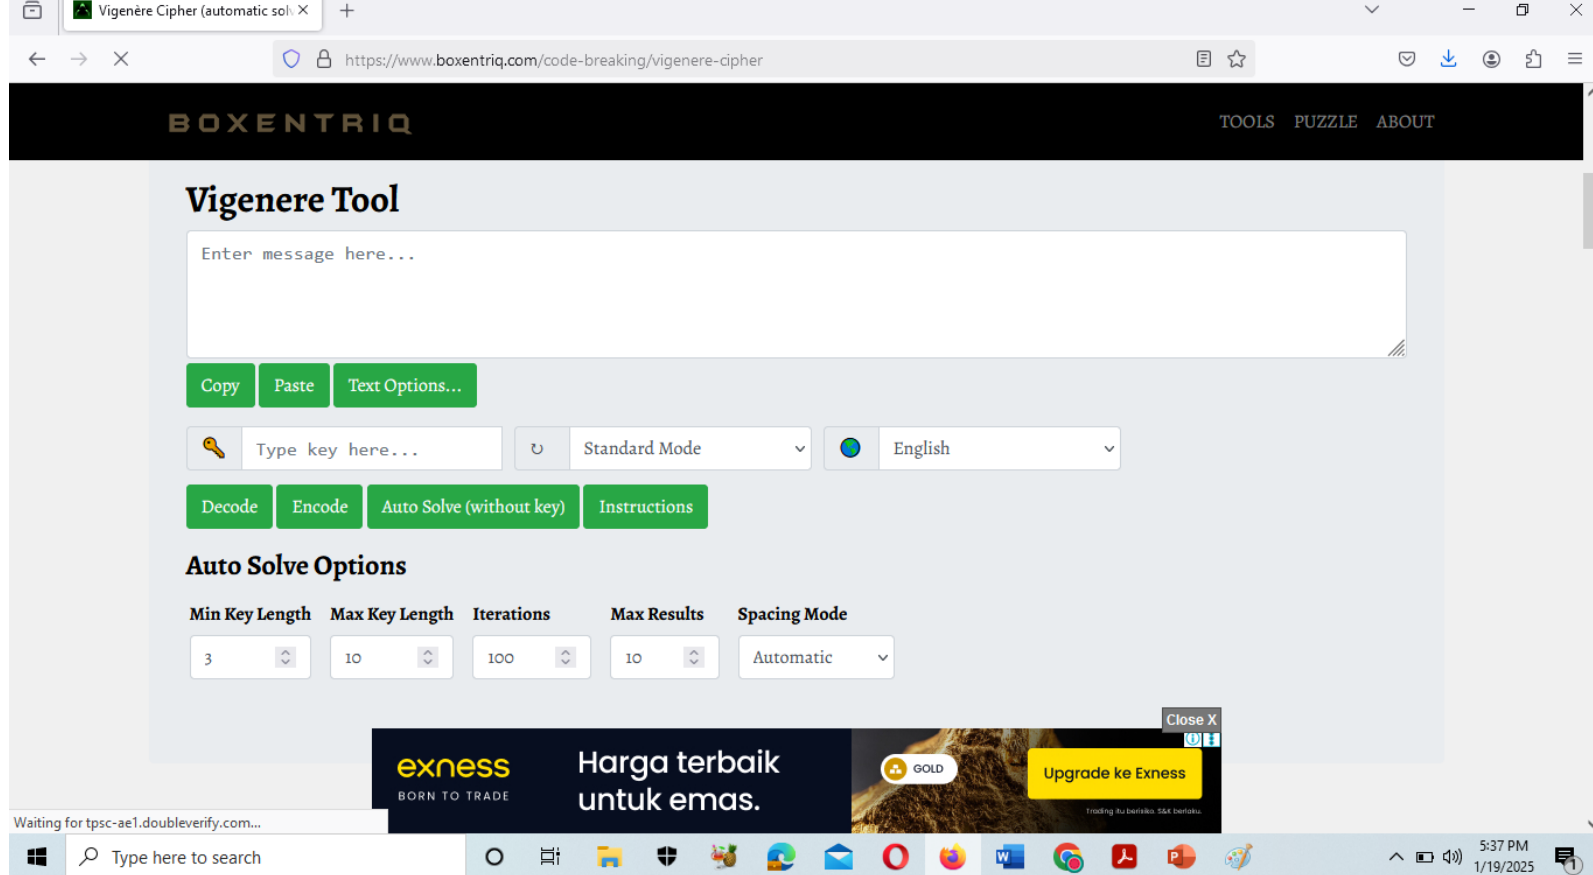
\includegraphics[width=174.30mm,height=240.57mm]{../../images/llm/page_042_img_01.png}%
\end{textblock*}

\end{document}
